%==================================================
% This is for generating a standalone sprint 1 plan
%==================================================
%\def\sphinxdocclass{report}
\documentclass[a4paper, 11pt]{report}
\usepackage[T1]{fontenc}
\usepackage[utf8]{inputenc}
\usepackage[english]{babel}
\usepackage{graphicx} % support graphics
\usepackage{hyperref} % links in the document
\usepackage{float} % position of figures
\usepackage{paralist} % inline lists
\usepackage{verbatim} % multiline comments
\usepackage[table]{xcolor} % table row coloring
\usepackage{booktabs} % Professional tables
\usepackage{tabularx} % Simple column stretching
\usepackage{multirow} % Row spanning
\usepackage{wrapfig} % Wrap text around figures
\usepackage{array}
\usepackage{listings}
\usepackage{color}
\usepackage{textcomp}
\usepackage[style=treenoname,subentrycounter,numberedsection, 
        section=chapter, acronym]{glossaries}
% new for userdoc
% \usepackage{times}
% \usepackage{longtable}
% \usepackage{sphinx}
% \usepackage[Bjarne]{fncychap}
% \usepackage[T1]{fontenc}
% \DeclareUnicodeCharacter{00A0}{\nobreakspace}
% \usepackage{fancyvrb}
% \usepackage{fancybox}
% \usepackage{subsections}
% \setcounter{secnumdepth}{5}
\usepackage{standalone}

\newcommand\codeHighlight[1]{\textcolor[rgb]{1,0,0}{\textbf{#1}}}

\definecolor{listinggray}{gray}{0.9}
\definecolor{lbcolor}{rgb}{0.9,0.9,0.9}

\lstset{
    backgroundcolor=\color{lbcolor},
    tabsize=4,
    rulecolor=,
    language=C,
    basicstyle=\footnotesize,
    upquote=true,
    aboveskip={1.5\baselineskip},
    columns=fixed,
    showstringspaces=false,
    extendedchars=true,
    breaklines=true,
    prebreak = \raisebox{0ex}[0ex][0ex]{\ensuremath{\hookleftarrow}},
    frame=single,
    showtabs=false,
    showspaces=false,
    showstringspaces=false,
    identifierstyle=\ttfamily,
    keywordstyle=\color[rgb]{0,0,1},
    commentstyle=\color[rgb]{0.133,0.545,0.133},
    stringstyle=\color[rgb]{0.627,0.126,0.941},
}

% Generated by Sphinx.
% \def\sphinxdocclass{report}
% \documentclass[letterpaper,10pt,english]{sphinxmanual}
% \usepackage[utf8]{inputenc}
\DeclareUnicodeCharacter{00A0}{\nobreakspace}
% \usepackage[T1]{fontenc}
% \usepackage{babel}
% \usepackage{times}
% \usepackage[Bjarne]{fncychap}
% \usepackage{longtable}
% \usepackage{sphinx}
% \usepackage{multirow}

\newcommand{\strong}[1]{{\bf #1}}
\newcommand{\code}[1]{\texttt{#1}}
\newcommand{\bfcode}[1]{\code{\bfseries#1}}
\usepackage{tabulary}
\usepackage{fancyvrb}
\usepackage{fancybox}
\usepackage{parskip}
\usepackage{hypcap}

% Notices / Admonitions
%
% \newlength{\py@noticelength}
% 
% \newcommand{\py@heavybox}{
%   \setlength{\fboxrule}{1pt}
%   \setlength{\fboxsep}{6pt}
%   \setlength{\py@noticelength}{\linewidth}
%   \addtolength{\py@noticelength}{-2\fboxsep}
%   \addtolength{\py@noticelength}{-2\fboxrule}
%   %\setlength{\shadowsize}{3pt}
%   \Sbox
%   \minipage{\py@noticelength}
% }
% \newcommand{\py@endheavybox}{
%   \endminipage
%   \endSbox
%   \fbox{\TheSbox}
% }
% 
% \newcommand{\py@lightbox}{{%
%   \setlength\parskip{0pt}\par
%   \rule[0ex]{\linewidth}{0.5pt}%
%   \par\vspace{-0.5ex}%
%   }}
% \newcommand{\py@endlightbox}{{%
%   \setlength{\parskip}{0pt}%
%   \par\rule[0.5ex]{\linewidth}{0.5pt}%
%   \par\vspace{-0.5ex}%
%   }}
% 
% % Some are quite plain:
% \newcommand{\py@noticestart@note}{\py@lightbox}
% \newcommand{\py@noticeend@note}{\py@endlightbox}
% \newcommand{\py@noticestart@hint}{\py@lightbox}
% \newcommand{\py@noticeend@hint}{\py@endlightbox}
% \newcommand{\py@noticestart@important}{\py@lightbox}
% \newcommand{\py@noticeend@important}{\py@endlightbox}
% \newcommand{\py@noticestart@tip}{\py@lightbox}
% \newcommand{\py@noticeend@tip}{\py@endlightbox}
% 
% % Others gets more visible distinction:
% \newcommand{\py@noticestart@warning}{\py@heavybox}
% \newcommand{\py@noticeend@warning}{\py@endheavybox}
% \newcommand{\py@noticestart@caution}{\py@heavybox}
% \newcommand{\py@noticeend@caution}{\py@endheavybox}
% \newcommand{\py@noticestart@attention}{\py@heavybox}
% \newcommand{\py@noticeend@attention}{\py@endheavybox}
% \newcommand{\py@noticestart@danger}{\py@heavybox}
% \newcommand{\py@noticeend@danger}{\py@endheavybox}
% \newcommand{\py@noticestart@error}{\py@heavybox}
% \newcommand{\py@noticeend@error}{\py@endheavybox}
% 
% \newenvironment{notice}[2]{
%   \def\py@noticetype{#1}
%   \csname py@noticestart@#1\endcsname
%   \strong{#2}
% }{\csname py@noticeend@\py@noticetype\endcsname}

% {fulllineitems} is the main environment for object descriptions.
%
% \newcommand{\py@itemnewline}[1]{%
%   \@tempdima\linewidth%
%   \advance\@tempdima \leftmargin\makebox[\@tempdima][l]{#1}%
% }
% 
\newenvironment{fulllineitems}{
%   \begin{list}{}{\labelwidth \leftmargin \labelsep 0pt
%                  \rightmargin 0pt \topsep -\parskip \partopsep \parskip
%                  \itemsep -\parsep
%                  \let\makelabel=\py@itemnewline}
% }{\end{list}}
}
\newcommand{\pysigline}[1]{\item[#1]\nopagebreak}

% 
\makeatletter
\def\PYG@reset{\let\PYG@it=\relax \let\PYG@bf=\relax%
    \let\PYG@ul=\relax \let\PYG@tc=\relax%
    \let\PYG@bc=\relax \let\PYG@ff=\relax}
\def\PYG@tok#1{\csname PYG@tok@#1\endcsname}
\def\PYG@toks#1+{\ifx\relax#1\empty\else%
    \PYG@tok{#1}\expandafter\PYG@toks\fi}
\def\PYG@do#1{\PYG@bc{\PYG@tc{\PYG@ul{%
    \PYG@it{\PYG@bf{\PYG@ff{#1}}}}}}}
\def\PYG#1#2{\PYG@reset\PYG@toks#1+\relax+\PYG@do{#2}}

\def\PYG@tok@gd{\def\PYG@tc##1{\textcolor[rgb]{0.63,0.00,0.00}{##1}}}
\def\PYG@tok@gu{\let\PYG@bf=\textbf\def\PYG@tc##1{\textcolor[rgb]{0.50,0.00,0.50}{##1}}}
\def\PYG@tok@gt{\def\PYG@tc##1{\textcolor[rgb]{0.00,0.25,0.82}{##1}}}
\def\PYG@tok@gs{\let\PYG@bf=\textbf}
\def\PYG@tok@gr{\def\PYG@tc##1{\textcolor[rgb]{1.00,0.00,0.00}{##1}}}
\def\PYG@tok@cm{\let\PYG@it=\textit\def\PYG@tc##1{\textcolor[rgb]{0.25,0.50,0.56}{##1}}}
\def\PYG@tok@vg{\def\PYG@tc##1{\textcolor[rgb]{0.73,0.38,0.84}{##1}}}
\def\PYG@tok@m{\def\PYG@tc##1{\textcolor[rgb]{0.13,0.50,0.31}{##1}}}
\def\PYG@tok@mh{\def\PYG@tc##1{\textcolor[rgb]{0.13,0.50,0.31}{##1}}}
\def\PYG@tok@cs{\def\PYG@tc##1{\textcolor[rgb]{0.25,0.50,0.56}{##1}}\def\PYG@bc##1{\colorbox[rgb]{1.00,0.94,0.94}{##1}}}
\def\PYG@tok@ge{\let\PYG@it=\textit}
\def\PYG@tok@vc{\def\PYG@tc##1{\textcolor[rgb]{0.73,0.38,0.84}{##1}}}
\def\PYG@tok@il{\def\PYG@tc##1{\textcolor[rgb]{0.13,0.50,0.31}{##1}}}
\def\PYG@tok@go{\def\PYG@tc##1{\textcolor[rgb]{0.19,0.19,0.19}{##1}}}
\def\PYG@tok@cp{\def\PYG@tc##1{\textcolor[rgb]{0.00,0.44,0.13}{##1}}}
\def\PYG@tok@gi{\def\PYG@tc##1{\textcolor[rgb]{0.00,0.63,0.00}{##1}}}
\def\PYG@tok@gh{\let\PYG@bf=\textbf\def\PYG@tc##1{\textcolor[rgb]{0.00,0.00,0.50}{##1}}}
\def\PYG@tok@ni{\let\PYG@bf=\textbf\def\PYG@tc##1{\textcolor[rgb]{0.84,0.33,0.22}{##1}}}
\def\PYG@tok@nl{\let\PYG@bf=\textbf\def\PYG@tc##1{\textcolor[rgb]{0.00,0.13,0.44}{##1}}}
\def\PYG@tok@nn{\let\PYG@bf=\textbf\def\PYG@tc##1{\textcolor[rgb]{0.05,0.52,0.71}{##1}}}
\def\PYG@tok@no{\def\PYG@tc##1{\textcolor[rgb]{0.38,0.68,0.84}{##1}}}
\def\PYG@tok@na{\def\PYG@tc##1{\textcolor[rgb]{0.25,0.44,0.63}{##1}}}
\def\PYG@tok@nb{\def\PYG@tc##1{\textcolor[rgb]{0.00,0.44,0.13}{##1}}}
\def\PYG@tok@nc{\let\PYG@bf=\textbf\def\PYG@tc##1{\textcolor[rgb]{0.05,0.52,0.71}{##1}}}
\def\PYG@tok@nd{\let\PYG@bf=\textbf\def\PYG@tc##1{\textcolor[rgb]{0.33,0.33,0.33}{##1}}}
\def\PYG@tok@ne{\def\PYG@tc##1{\textcolor[rgb]{0.00,0.44,0.13}{##1}}}
\def\PYG@tok@nf{\def\PYG@tc##1{\textcolor[rgb]{0.02,0.16,0.49}{##1}}}
\def\PYG@tok@si{\let\PYG@it=\textit\def\PYG@tc##1{\textcolor[rgb]{0.44,0.63,0.82}{##1}}}
\def\PYG@tok@s2{\def\PYG@tc##1{\textcolor[rgb]{0.25,0.44,0.63}{##1}}}
\def\PYG@tok@vi{\def\PYG@tc##1{\textcolor[rgb]{0.73,0.38,0.84}{##1}}}
\def\PYG@tok@nt{\let\PYG@bf=\textbf\def\PYG@tc##1{\textcolor[rgb]{0.02,0.16,0.45}{##1}}}
\def\PYG@tok@nv{\def\PYG@tc##1{\textcolor[rgb]{0.73,0.38,0.84}{##1}}}
\def\PYG@tok@s1{\def\PYG@tc##1{\textcolor[rgb]{0.25,0.44,0.63}{##1}}}
\def\PYG@tok@gp{\let\PYG@bf=\textbf\def\PYG@tc##1{\textcolor[rgb]{0.78,0.36,0.04}{##1}}}
\def\PYG@tok@sh{\def\PYG@tc##1{\textcolor[rgb]{0.25,0.44,0.63}{##1}}}
\def\PYG@tok@ow{\let\PYG@bf=\textbf\def\PYG@tc##1{\textcolor[rgb]{0.00,0.44,0.13}{##1}}}
\def\PYG@tok@sx{\def\PYG@tc##1{\textcolor[rgb]{0.78,0.36,0.04}{##1}}}
\def\PYG@tok@bp{\def\PYG@tc##1{\textcolor[rgb]{0.00,0.44,0.13}{##1}}}
\def\PYG@tok@c1{\let\PYG@it=\textit\def\PYG@tc##1{\textcolor[rgb]{0.25,0.50,0.56}{##1}}}
\def\PYG@tok@kc{\let\PYG@bf=\textbf\def\PYG@tc##1{\textcolor[rgb]{0.00,0.44,0.13}{##1}}}
\def\PYG@tok@c{\let\PYG@it=\textit\def\PYG@tc##1{\textcolor[rgb]{0.25,0.50,0.56}{##1}}}
\def\PYG@tok@mf{\def\PYG@tc##1{\textcolor[rgb]{0.13,0.50,0.31}{##1}}}
\def\PYG@tok@err{\def\PYG@bc##1{\fcolorbox[rgb]{1.00,0.00,0.00}{1,1,1}{##1}}}
\def\PYG@tok@kd{\let\PYG@bf=\textbf\def\PYG@tc##1{\textcolor[rgb]{0.00,0.44,0.13}{##1}}}
\def\PYG@tok@ss{\def\PYG@tc##1{\textcolor[rgb]{0.32,0.47,0.09}{##1}}}
\def\PYG@tok@sr{\def\PYG@tc##1{\textcolor[rgb]{0.14,0.33,0.53}{##1}}}
\def\PYG@tok@mo{\def\PYG@tc##1{\textcolor[rgb]{0.13,0.50,0.31}{##1}}}
\def\PYG@tok@mi{\def\PYG@tc##1{\textcolor[rgb]{0.13,0.50,0.31}{##1}}}
\def\PYG@tok@kn{\let\PYG@bf=\textbf\def\PYG@tc##1{\textcolor[rgb]{0.00,0.44,0.13}{##1}}}
\def\PYG@tok@o{\def\PYG@tc##1{\textcolor[rgb]{0.40,0.40,0.40}{##1}}}
\def\PYG@tok@kr{\let\PYG@bf=\textbf\def\PYG@tc##1{\textcolor[rgb]{0.00,0.44,0.13}{##1}}}
\def\PYG@tok@s{\def\PYG@tc##1{\textcolor[rgb]{0.25,0.44,0.63}{##1}}}
\def\PYG@tok@kp{\def\PYG@tc##1{\textcolor[rgb]{0.00,0.44,0.13}{##1}}}
\def\PYG@tok@w{\def\PYG@tc##1{\textcolor[rgb]{0.73,0.73,0.73}{##1}}}
\def\PYG@tok@kt{\def\PYG@tc##1{\textcolor[rgb]{0.56,0.13,0.00}{##1}}}
\def\PYG@tok@sc{\def\PYG@tc##1{\textcolor[rgb]{0.25,0.44,0.63}{##1}}}
\def\PYG@tok@sb{\def\PYG@tc##1{\textcolor[rgb]{0.25,0.44,0.63}{##1}}}
\def\PYG@tok@k{\let\PYG@bf=\textbf\def\PYG@tc##1{\textcolor[rgb]{0.00,0.44,0.13}{##1}}}
\def\PYG@tok@se{\let\PYG@bf=\textbf\def\PYG@tc##1{\textcolor[rgb]{0.25,0.44,0.63}{##1}}}
\def\PYG@tok@sd{\let\PYG@it=\textit\def\PYG@tc##1{\textcolor[rgb]{0.25,0.44,0.63}{##1}}}

\def\PYGZbs{\char`\\}
\def\PYGZus{\char`\_}
\def\PYGZob{\char`\{}
\def\PYGZcb{\char`\}}
\def\PYGZca{\char`\^}
\def\PYGZsh{\char`\#}
\def\PYGZpc{\char`\%}
\def\PYGZdl{\char`\$}
\def\PYGZti{\char`\~}
% for compatibility with earlier versions
\def\PYGZat{@}
\def\PYGZlb{[}
\def\PYGZrb{]}
\makeatother

% Configure links in pdfs
\hypersetup{
    bookmarksopen=false, % Hide bookmarks menu
    colorlinks=true, % Don't wrap links in colored boxes
}

\title{User and Developer Manual}
\author{Kpro group 9}
\date{\today}

\begin{document}
%\maketitle
%\tableofcontents
\begin{standalone}
    % Generated by Sphinx.
\def\sphinxdocclass{report}
\documentclass[A4paper,10pt,english]{sphinxmanual}
\usepackage[utf8]{inputenc}
\DeclareUnicodeCharacter{00A0}{\nobreakspace}
\usepackage[T1]{fontenc}
\usepackage{babel}
\usepackage{times}
\usepackage[Bjarne]{fncychap}
\usepackage{longtable}
\usepackage{sphinx}
\usepackage{multirow}


\title{CSjark Documentation}
\date{November 16, 2011}
\release{0.3.2}
\author{Erik Bergersen \and Jaroslav Fibichr \and Sondre Johan Mannsverk \and Terje Snarby \and Even Wiik Thomassen \and Lars Solvoll Tønder \and Sigurd Wien}
\newcommand{\sphinxlogo}{}
\renewcommand{\releasename}{Release}
\makeindex

\makeatletter
\def\PYG@reset{\let\PYG@it=\relax \let\PYG@bf=\relax%
    \let\PYG@ul=\relax \let\PYG@tc=\relax%
    \let\PYG@bc=\relax \let\PYG@ff=\relax}
\def\PYG@tok#1{\csname PYG@tok@#1\endcsname}
\def\PYG@toks#1+{\ifx\relax#1\empty\else%
    \PYG@tok{#1}\expandafter\PYG@toks\fi}
\def\PYG@do#1{\PYG@bc{\PYG@tc{\PYG@ul{%
    \PYG@it{\PYG@bf{\PYG@ff{#1}}}}}}}
\def\PYG#1#2{\PYG@reset\PYG@toks#1+\relax+\PYG@do{#2}}

\def\PYG@tok@gd{\def\PYG@tc##1{\textcolor[rgb]{0.63,0.00,0.00}{##1}}}
\def\PYG@tok@gu{\let\PYG@bf=\textbf\def\PYG@tc##1{\textcolor[rgb]{0.50,0.00,0.50}{##1}}}
\def\PYG@tok@gt{\def\PYG@tc##1{\textcolor[rgb]{0.00,0.25,0.82}{##1}}}
\def\PYG@tok@gs{\let\PYG@bf=\textbf}
\def\PYG@tok@gr{\def\PYG@tc##1{\textcolor[rgb]{1.00,0.00,0.00}{##1}}}
\def\PYG@tok@cm{\let\PYG@it=\textit\def\PYG@tc##1{\textcolor[rgb]{0.25,0.50,0.56}{##1}}}
\def\PYG@tok@vg{\def\PYG@tc##1{\textcolor[rgb]{0.73,0.38,0.84}{##1}}}
\def\PYG@tok@m{\def\PYG@tc##1{\textcolor[rgb]{0.13,0.50,0.31}{##1}}}
\def\PYG@tok@mh{\def\PYG@tc##1{\textcolor[rgb]{0.13,0.50,0.31}{##1}}}
\def\PYG@tok@cs{\def\PYG@tc##1{\textcolor[rgb]{0.25,0.50,0.56}{##1}}\def\PYG@bc##1{\colorbox[rgb]{1.00,0.94,0.94}{##1}}}
\def\PYG@tok@ge{\let\PYG@it=\textit}
\def\PYG@tok@vc{\def\PYG@tc##1{\textcolor[rgb]{0.73,0.38,0.84}{##1}}}
\def\PYG@tok@il{\def\PYG@tc##1{\textcolor[rgb]{0.13,0.50,0.31}{##1}}}
\def\PYG@tok@go{\def\PYG@tc##1{\textcolor[rgb]{0.19,0.19,0.19}{##1}}}
\def\PYG@tok@cp{\def\PYG@tc##1{\textcolor[rgb]{0.00,0.44,0.13}{##1}}}
\def\PYG@tok@gi{\def\PYG@tc##1{\textcolor[rgb]{0.00,0.63,0.00}{##1}}}
\def\PYG@tok@gh{\let\PYG@bf=\textbf\def\PYG@tc##1{\textcolor[rgb]{0.00,0.00,0.50}{##1}}}
\def\PYG@tok@ni{\let\PYG@bf=\textbf\def\PYG@tc##1{\textcolor[rgb]{0.84,0.33,0.22}{##1}}}
\def\PYG@tok@nl{\let\PYG@bf=\textbf\def\PYG@tc##1{\textcolor[rgb]{0.00,0.13,0.44}{##1}}}
\def\PYG@tok@nn{\let\PYG@bf=\textbf\def\PYG@tc##1{\textcolor[rgb]{0.05,0.52,0.71}{##1}}}
\def\PYG@tok@no{\def\PYG@tc##1{\textcolor[rgb]{0.38,0.68,0.84}{##1}}}
\def\PYG@tok@na{\def\PYG@tc##1{\textcolor[rgb]{0.25,0.44,0.63}{##1}}}
\def\PYG@tok@nb{\def\PYG@tc##1{\textcolor[rgb]{0.00,0.44,0.13}{##1}}}
\def\PYG@tok@nc{\let\PYG@bf=\textbf\def\PYG@tc##1{\textcolor[rgb]{0.05,0.52,0.71}{##1}}}
\def\PYG@tok@nd{\let\PYG@bf=\textbf\def\PYG@tc##1{\textcolor[rgb]{0.33,0.33,0.33}{##1}}}
\def\PYG@tok@ne{\def\PYG@tc##1{\textcolor[rgb]{0.00,0.44,0.13}{##1}}}
\def\PYG@tok@nf{\def\PYG@tc##1{\textcolor[rgb]{0.02,0.16,0.49}{##1}}}
\def\PYG@tok@si{\let\PYG@it=\textit\def\PYG@tc##1{\textcolor[rgb]{0.44,0.63,0.82}{##1}}}
\def\PYG@tok@s2{\def\PYG@tc##1{\textcolor[rgb]{0.25,0.44,0.63}{##1}}}
\def\PYG@tok@vi{\def\PYG@tc##1{\textcolor[rgb]{0.73,0.38,0.84}{##1}}}
\def\PYG@tok@nt{\let\PYG@bf=\textbf\def\PYG@tc##1{\textcolor[rgb]{0.02,0.16,0.45}{##1}}}
\def\PYG@tok@nv{\def\PYG@tc##1{\textcolor[rgb]{0.73,0.38,0.84}{##1}}}
\def\PYG@tok@s1{\def\PYG@tc##1{\textcolor[rgb]{0.25,0.44,0.63}{##1}}}
\def\PYG@tok@gp{\let\PYG@bf=\textbf\def\PYG@tc##1{\textcolor[rgb]{0.78,0.36,0.04}{##1}}}
\def\PYG@tok@sh{\def\PYG@tc##1{\textcolor[rgb]{0.25,0.44,0.63}{##1}}}
\def\PYG@tok@ow{\let\PYG@bf=\textbf\def\PYG@tc##1{\textcolor[rgb]{0.00,0.44,0.13}{##1}}}
\def\PYG@tok@sx{\def\PYG@tc##1{\textcolor[rgb]{0.78,0.36,0.04}{##1}}}
\def\PYG@tok@bp{\def\PYG@tc##1{\textcolor[rgb]{0.00,0.44,0.13}{##1}}}
\def\PYG@tok@c1{\let\PYG@it=\textit\def\PYG@tc##1{\textcolor[rgb]{0.25,0.50,0.56}{##1}}}
\def\PYG@tok@kc{\let\PYG@bf=\textbf\def\PYG@tc##1{\textcolor[rgb]{0.00,0.44,0.13}{##1}}}
\def\PYG@tok@c{\let\PYG@it=\textit\def\PYG@tc##1{\textcolor[rgb]{0.25,0.50,0.56}{##1}}}
\def\PYG@tok@mf{\def\PYG@tc##1{\textcolor[rgb]{0.13,0.50,0.31}{##1}}}
\def\PYG@tok@err{\def\PYG@bc##1{\fcolorbox[rgb]{1.00,0.00,0.00}{1,1,1}{##1}}}
\def\PYG@tok@kd{\let\PYG@bf=\textbf\def\PYG@tc##1{\textcolor[rgb]{0.00,0.44,0.13}{##1}}}
\def\PYG@tok@ss{\def\PYG@tc##1{\textcolor[rgb]{0.32,0.47,0.09}{##1}}}
\def\PYG@tok@sr{\def\PYG@tc##1{\textcolor[rgb]{0.14,0.33,0.53}{##1}}}
\def\PYG@tok@mo{\def\PYG@tc##1{\textcolor[rgb]{0.13,0.50,0.31}{##1}}}
\def\PYG@tok@mi{\def\PYG@tc##1{\textcolor[rgb]{0.13,0.50,0.31}{##1}}}
\def\PYG@tok@kn{\let\PYG@bf=\textbf\def\PYG@tc##1{\textcolor[rgb]{0.00,0.44,0.13}{##1}}}
\def\PYG@tok@o{\def\PYG@tc##1{\textcolor[rgb]{0.40,0.40,0.40}{##1}}}
\def\PYG@tok@kr{\let\PYG@bf=\textbf\def\PYG@tc##1{\textcolor[rgb]{0.00,0.44,0.13}{##1}}}
\def\PYG@tok@s{\def\PYG@tc##1{\textcolor[rgb]{0.25,0.44,0.63}{##1}}}
\def\PYG@tok@kp{\def\PYG@tc##1{\textcolor[rgb]{0.00,0.44,0.13}{##1}}}
\def\PYG@tok@w{\def\PYG@tc##1{\textcolor[rgb]{0.73,0.73,0.73}{##1}}}
\def\PYG@tok@kt{\def\PYG@tc##1{\textcolor[rgb]{0.56,0.13,0.00}{##1}}}
\def\PYG@tok@sc{\def\PYG@tc##1{\textcolor[rgb]{0.25,0.44,0.63}{##1}}}
\def\PYG@tok@sb{\def\PYG@tc##1{\textcolor[rgb]{0.25,0.44,0.63}{##1}}}
\def\PYG@tok@k{\let\PYG@bf=\textbf\def\PYG@tc##1{\textcolor[rgb]{0.00,0.44,0.13}{##1}}}
\def\PYG@tok@se{\let\PYG@bf=\textbf\def\PYG@tc##1{\textcolor[rgb]{0.25,0.44,0.63}{##1}}}
\def\PYG@tok@sd{\let\PYG@it=\textit\def\PYG@tc##1{\textcolor[rgb]{0.25,0.44,0.63}{##1}}}

\def\PYGZbs{\char`\\}
\def\PYGZus{\char`\_}
\def\PYGZob{\char`\{}
\def\PYGZcb{\char`\}}
\def\PYGZca{\char`\^}
\def\PYGZsh{\char`\#}
\def\PYGZpc{\char`\%}
\def\PYGZdl{\char`\$}
\def\PYGZti{\char`\~}
% for compatibility with earlier versions
\def\PYGZat{@}
\def\PYGZlb{[}
\def\PYGZrb{]}
\makeatother

%


\begin{document}

% \maketitle
% \tableofcontents
\phantomsection\label{index::doc}

\newpage    

CSjark is a tool for generating Lua dissectors from C struct definitions to use with Wireshark. Wireshark is a leading tool for capturing and analysing network traffic. The goal with the dissectors is to make Wireshark able to nicely display the values of a struct sent over the network, along with member names and type. This can be a powerful tool for debugging C programs that communicates with strucs over the network.

For more information about Wireshark please visit \href{http://www.wireshark.org}{Wireshark website}.


\section{User Documentation}
\label{index:user-documentation}\label{index:welcome-to-csjark-s-documentation}

\subsection{Installing CSjark}
\label{user/install::doc}\label{user/install:installing-csjark}

\subsubsection{Dependencies}
\label{user/install:dependencies}
CSjark is written in Python 3.2, and therefore needs Python 3.2 (or later) to run. Latest implementation of Python can be downloaded from \href{http://www.python.org/}{Python website}. For installing please follow the instruction found there.

There are 4 third party dependencies to get CSjark working:
\begin{enumerate}
\item {} \begin{description}
\item[{\textbf{PLY} (Python Lex-Yacc)}] \leavevmode
PLY is an implementation of lex and yacc parsing tools for Python. It is required by pycparser. Instructions and further information can be found on the page linked above.

\begin{tabulary}{\linewidth}{|L|L|}
\hline

\textbf{Required version}
 & 
3.4
\\\hline

\textbf{Download location}
 & 
\href{http://www.dabeaz.com/ply/}{http://www.dabeaz.com/ply/}
\\\hline
\end{tabulary}


\end{description}

\item {} \begin{description}
\item[{\textbf{pycpaser}}] \leavevmode
\href{http://code.google.com/p/pycparser/}{Pycparser} is a C parser (and AST generator) implemented in Python. Due to the continuous development, CSjark requires the latest development version (not the release version).

\begin{tabulary}{\linewidth}{|L|L|}
\hline

\textbf{Required version}
 & 
latest development version from pycparser repository
\\\hline

\textbf{Download location}
 & 
pycparser repository: \href{http://code.google.com/p/pycparser/source/checkout}{http://code.google.com/p/pycparser/source/checkout}
\\\hline
\end{tabulary}


\end{description}

\item {} \begin{description}
\item[{\textbf{C  preprocessor}}] \leavevmode
CSjark requires a C-preprocessor. The way how to get one depends on operating system used by the user:

\begin{tabulary}{\linewidth}{|L|L|}
\hline

\textbf{Windows}
 & 
Bundled with CSjark.
\\\hline

\textbf{OS X, Linux, Solaris}
 & 
Needs to be installed separately. For example, as a part of \href{http://gcc.gnu.org/}{GCC}
\\\hline
\end{tabulary}


\end{description}

\item {} 
\textbf{pyYAML}
\begin{quote}

\href{http://pyyaml.org/wiki/PyYAML}{pyYAML} is a YAML parser and emitter for the Python programming language. \href{http://yaml.org/}{YAML} is a standard used to specify configurations to CSjark. The website includes both a way to download the software and also instructions of how to install it.

\begin{tabulary}{\linewidth}{|L|L|}
\hline

\textbf{Required version}
 & 
3.10
\\\hline

\textbf{Download location}
 & 
\href{http://pyyaml.org/wiki/PyYAML}{http://pyyaml.org/wiki/PyYAML}
\\\hline
\end{tabulary}

\end{quote}

\end{enumerate}


\subsubsection{Wireshark}
\label{user/install:ws}\label{user/install:wireshark}
\href{http://www.wireshark.org/}{Wireshark} is an open source protocol analyzer which can use the Lua dissectors generated by CSjark. To get the proper integration of Lua dissectors, the latest development version of Wireshark is required.

\begin{tabulary}{\linewidth}{|L|L|}
\hline

\textbf{Required version}
 & 
1.7 dev (build 39446 or newer)
\\\hline

\textbf{Download location}
 & 
\href{http://www.wireshark.org/download/automated/}{http://www.wireshark.org/download/automated/}, on the page, browse for the required platform version
\\\hline
\end{tabulary}



\subsubsection{CSjark}
\label{user/install:csjark}
CSjark can be obtained at git CSjark repository: \href{https://github.com/eventh/kpro9/}{https://github.com/eventh/kpro9/}.
CSjark itself requires no installation. After the steps described in the dependencies section is completed. It can be ran by opening a terminal, navigating to the directory containing \code{cshark.py} and invoking as described in section {\hyperref[user/use:use]{\emph{Using CSjark}}}.


\subsection{Using CSjark}
\label{user/use:using-csjark}\label{user/use:use}\label{user/use::doc}
CSjark can be invoked by running the \code{csjark.py} script. The arguments must be specified according to:

\begin{Verbatim}[commandchars=\\\{\}]
csjark.py [-h] [-v] [-d] [-s] [-f [header [header ...]]]
          [-c [config [config ...]]] [-x [path [path ...]]]
          [-o [output]] [-p] [-n] [-C [cpp]] [-i [header [header ...]]]
          [-I [directory [directory ...]]]
          [-D [name=definition [name=definition ...]]]
          [-U [name [name ...]]] [-A [argument [argument ...]]]
          [header] [config]
\end{Verbatim}

The arguments here specify the following:
\begin{description}
\item[{\code{header}}] \leavevmode
a c header file to parse.

\item[{\code{config}}] \leavevmode
a configuration file to parse.

\end{description}

\textbf{Optional arguments:}
\begin{quote}

\begin{tabulary}{\textwidth}{|L|L|}
\hline

\code{-h, -{-}help}
 & 
Show a help message and exit.
\\\hline

\code{-v, -{-}verbose}
 & 
Print detailed information.
\\\hline

\code{-d, -{-}debug}
 & 
Print debugging information.
\\\hline

\code{-s, -{-}strict}
 & 
Only generate dissectors for known structs.
\\\hline

\code{-f {[}header {[}header ...{]}{]}, -{-}file {[}header {[}header ...{]}{]}}
 & 
Specifies that CSjark should look for struct definitions in the \code{header} files.
\\\hline

\code{-c {[}config {[}config ...{]}{]}, -{-}config {[}config {[}config ...{]}{]}}
 & 
Specifies that the program should use the \code{config} files as configuration.
\\\hline

\code{-x {[}path {[}path ...{]}{]}, -{-}exclude {[}path {[}path ...{]}{]}}
 & 
File or folders to exclude from parsing
\\\hline

\code{-o {[}output{]}, -{-}output {[}output{]}}
 & 
Writes the output to the specified file \code{output}.
\\\hline

\code{-p, -{-}placeholders}
 & 
Generate placeholder config file for unknown structs
\\\hline

\code{-n, -{-}nocpp}
 & 
Disables the C pre-processor.
\\\hline

\code{-C {[}cpp{]}, -{-}CPP {[}cpp{]}}
 & 
Specifies which preprocessor to use.
\\\hline

\code{-i {[}header {[}header ...{]}{]}, -{-}include {[}header {[}header ...{]}{]}}
 & 
Process file as Cpp \code{\#include "file"} directive
\\\hline

\code{-I {[}directory {[}directory ...{]}{]}, -{-}Includes {[}directory {[}directory ...{]}{]}}
 & 
Directories to be searched for Cpp includes
\\\hline

\code{-D {[}name=definition {[}name=definition ...{]}{]}, -{-}Define {[}name=definition {[}name=definition ...{]}{]}}
 & 
Predefine name as a Cpp macro
\\\hline

\code{-U {[}name {[}name ...{]}{]}, -{-}Undefine {[}name {[}name ...{]}{]}}
 & 
Cancel any previous Cpp definition of name
\\\hline

\code{-A {[}argument {[}argument ...{]}{]}, -{-}Additional {[}argument {[}argument ...{]}{]}}
 & 
Any additional C preprocessor arguments
\\\hline
\end{tabulary}

\end{quote}

\textbf{Example usage:}

\begin{Verbatim}[commandchars=\\\{\}]
python csjark.py -v headerfile.h configfile.yml
\end{Verbatim}

\textbf{Batch mode}

One of the most important features of CSjark is processing multiple C header files in one run. That can be easily achieved by specifying a directory instead of a single file as command line argument (see above):

\begin{Verbatim}[commandchars=\\\{\}]
python csjark.py headers configs
\end{Verbatim}

In batch mode, CSjark only generates dissectors for structs that have a configuration file with an ID (see section {\hyperref[user/config:ids]{\emph{Dissector message ID}}} for information how to specify dissector message ID), and for structs that depend on other structs. This speeds up the generation of dissectors, since it only generates dissectors that Wireshark can use.


\subsection{Using the generated Lua files in Wireshark}
\label{user/use_ws:using-the-generated-lua-files-in-wireshark}\label{user/use_ws::doc}
These are the steps needed to use a Lua dissector generated by CSjark with Wireshark.
\begin{enumerate}
\item {} 
Get the latest version of Wireshark as described in the installation section {\hyperref[user/install:ws]{\emph{Wireshark}}}.

\item {} 
Locate the Personal configuration and the Personal Plugins directories. To do this, start Wireshark and click on \code{Help} in the menubar and then on \code{About Wireshark}. This should bring up the About Wireshark dialog. From there, navigate to the \code{Folders} tab. Locate folders \code{Personal configuration} and \code{Personal Plugins} and note their paths (see below).

\end{enumerate}

{\hfill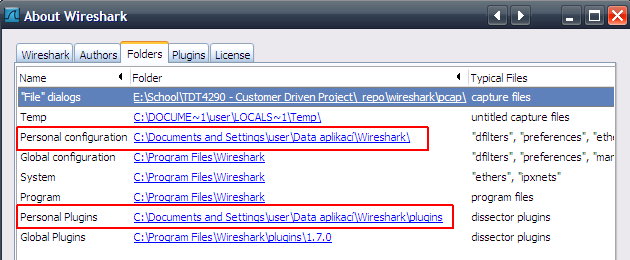
\includegraphics[width=\textwidth]{img/ws_about_folders.png}\hfill}
\begin{quote}
\begin{itemize}
\item {} 
on Linux/Unix system it may be  \code{\textasciitilde{}/.wireshark/} and  \code{\textasciitilde{}/.wireshark/plugins/}

\item {} \begin{description}
\item[{on Windows it may be \code{C:\textbackslash{}Users\textbackslash{}*YourUserName*\textbackslash{}AppData\textbackslash{}Roaming\textbackslash{}Wireshark\textbackslash{}}}] \leavevmode
and \code{C:\textbackslash{}Users\textbackslash{}*YourUserName*\textbackslash{}AppData\textbackslash{}Roaming\textbackslash{}Wireshark\textbackslash{}plugins\textbackslash{}}

\end{description}

\end{itemize}

If the folders does not exist, create them.
\end{quote}
\begin{enumerate}
\setcounter{enumi}{2}
\item {} 
Copy CSjark generated file \code{luastructs.lua} into the \code{Personal configuration} folder located in step 1.

\item {} 
Copy CSjark generated Lua dissectors into the \code{Personal Plugins} folder located in step 1.

\item {} 
Open the \code{init.lua} in the \code{Personal configuration} folder located in step 1. Insert the following code:

\begin{Verbatim}[commandchars=\\\{\}]
dofile("luastructs.lua")
\end{Verbatim}

\end{enumerate}
\begin{quote}

This ensures that the \code{luastructs.lua} is loaded before all other Lua scripts.
\end{quote}
\begin{enumerate}
\setcounter{enumi}{5}
\item {} \begin{description}
\item[{Restart Wireshark.}] \leavevmode
To check that the scripts are loaded, navigate to \code{Help} -\textgreater{} \code{About} -\textgreater{} \code{Plugins}. The scripts should now appear in the list as ``lua script''.

\end{description}

\end{enumerate}

{\hfill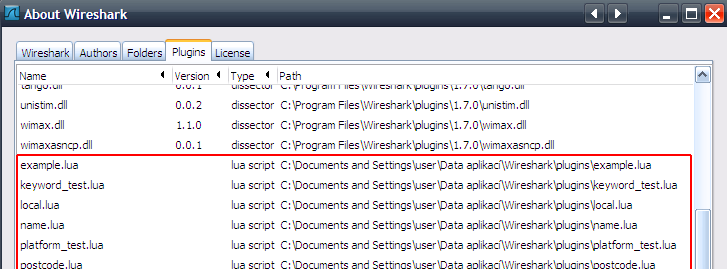
\includegraphics[width=\textwidth]{img/ws_about_plugins.png}\hfill}

To add further dissectors, only step 2, 5 and 6 needs to be repeated.

For further information on the Lua integration in Wireshark, please visit:
\href{http://www.wireshark.org/docs/wsug\_html\_chunked/wsluarm.html}{Lua Support in Wireshark}.


\subsection{Configuration}
\label{user/config:configuration}\label{user/config::doc}
Because there exists distinct requirements for flexibility of generating dissectors, CSjark supports configuration for various parts of the program. First, general parameters for utility running can be set up. This can be for example settings of variable sizes for different platforms or other parameters that could determine generating dissectors regardless actual C header file. Second, each individual C struct can be treated in different way. For example, value of specific struct member can be checked for being within specified limits.
\setbox0\vbox{
\begin{minipage}{0.95\linewidth}
\textbf{Contents}

\medskip

\begin{itemize}
\item {} 
{\hyperref[user/config:configuration]{Configuration}}
\begin{itemize}
\item {} 
{\hyperref[user/config:configuration-file-format-and-structure]{Configuration file format and structure}}

\item {} 
{\hyperref[user/config:struct-configuration]{Struct Configuration}}
\begin{itemize}
\item {} 
{\hyperref[user/config:value-ranges]{Value ranges}}

\item {} 
{\hyperref[user/config:value-explanations]{Value explanations}}
\begin{itemize}
\item {} 
{\hyperref[user/config:enums]{Enums}}

\item {} 
{\hyperref[user/config:bitstrings]{Bitstrings}}

\end{itemize}

\item {} 
{\hyperref[user/config:dissector-message-id]{Dissector message ID}}

\item {} 
{\hyperref[user/config:external-lua-dissectors]{External Lua dissectors}}
\begin{itemize}
\item {} 
{\hyperref[user/config:support-for-offset-and-value-in-lua-files]{Support for Offset and Value in Lua Files}}

\end{itemize}

\item {} 
{\hyperref[user/config:trailers]{Trailers}}

\item {} 
{\hyperref[user/config:custom-handling-of-data-types]{Custom handling of data types}}

\item {} 
{\hyperref[user/config:unknown-structs-handling]{Unknown structs handling}}

\end{itemize}

\item {} 
{\hyperref[user/config:options-configuration]{Options Configuration}}

\item {} 
{\hyperref[user/config:platform-specific-configuration]{Platform specific configuration}}

\end{itemize}

\end{itemize}
\end{minipage}}
\begin{center}\setlength{\fboxsep}{5pt}\shadowbox{\box0}\end{center}


\subsubsection{Configuration file format and structure}
\label{user/config:configuration-file-format-and-structure}
\textbf{Format}

The configuration files are written in \href{http://www.yaml.org/}{YAML} which is a data serialization format designed to be easy to read and write. Detailed specification can be found at \href{http://www.yaml.org/spec/1.2/spec.html}{YAML website}. The configuration must be put in a \code{filename.yml} file and specified when running CSjark as a command line argument (more about CLI in section {\hyperref[user/use:use]{\emph{Using CSjark}}}).

\textbf{Structure}

CSjark configuration files consist of 2 main parts. The first part is used for specifing all the configuration corresponding CSjark processing in general. More about CSjark options in {\hyperref[user/config:options-configuration]{Options Configuration}}. The second part contains configuration for individual C struct definitions. That is described in section {\hyperref[user/config:struct-configuration]{Struct Configuration}}.

The configuration file may have following strucuture:

\begin{Verbatim}[commandchars=\\\{\}]
Options:
  # there will be all your CSjark processing configuration
  use_cpp: True
  ...

Structs:
  # there will be a sequence of Struct definition configurations
  - name: struct1
    id: [10, 12, 14]
    # another struct1 config
  - name: struct2
    id: [11, 13, 15]
    # another struct2 config
\end{Verbatim}

\textbf{Automatic generation of configuration files}

Autogeneration of configuration file is a simple feature, that could save the user of the utility some time, since  the essential part of the configuration file is generated automatically.  The utility will only create a new file, containg the name of the struct and line to specifiy the ID for the dissector.  To generate the configuration file, the utility must be run with \code{-p} or \code{-{-}placeholders} as an option (see {\hyperref[user/use:use]{\emph{Using CSjark}}} for about CSjark CLI.

% \begin{notice}{note}{Note:}
One part of the configuration is held directly in the code. It represents the platform specific setup (file \code{platform.py}) - see {\hyperref[user/config:platform-specific-configuration]{Platform specific configuration}}.
% \end{notice}


\subsubsection{Struct Configuration}
\label{user/config:struct-configuration}
Each individual C struct processed by CSjark can be treated in different way. All the configuration settings must be done in the \code{Structs} section of the configuration file. Every Struct definition is one item of the sequence and may contain these attributes:

\begin{tabulary}{\linewidth}{|L|L|}
\hline
\textbf{
Attribute name
} & \textbf{
Description
}\\\hline

name
 & 
C struct name (required field)
\\\hline

id
 & 
Dissector message id - more in \emph{Dissector message ID}
\\\hline

description
 & 
Struct name displayed in Wireshark
\\\hline

size
 & 
Size of the struct in memory - more in {\hyperref[user/config:unknown-structs-handling]{Unknown structs handling}}
\\\hline

cnf
 & 
Conformance file name - more in {\hyperref[user/config:external-lua-dissectors]{External Lua dissectors}}
\\\hline

ranges
 & 
Value ranges limitations - more in {\hyperref[user/config:value-ranges]{Value ranges}}
\\\hline

enums
 & 
Enumeration definitions - more in {\hyperref[user/config:enums]{Enums}}
\\\hline

bitstrings
 & 
Bitstrings definitions - more in {\hyperref[user/config:bitstrings]{Bitstrings}}
\\\hline

trailers
 & 
Trailers definitions - more in {\hyperref[user/config:trailers]{Trailers}}
\\\hline

customs
 & 
Definitions for custom struct member handling - more in {\hyperref[user/config:custom-handling-of-data-types]{Custom handling of data types}}
\\\hline
\end{tabulary}



\paragraph{Value ranges}
\label{user/config:value-ranges}
Some variables may have a domain that is smaller than its given type. You could for example use an integer to describe percentage, which is a number between 0 and 100. It is possible to specify this to CSjark, so that the resulting dissector will tell Wireshark if the values are in the specified range or not. Value ranges are defined by the following syntax:

\begin{Verbatim}[commandchars=\\\{\}]
Structs:
  - name: "Name of the struct"
    id: 989
    ranges:
        - member | type: "Name of struct member / type"
          min: "Lowest allowed value"
          max: "Highest allowed value"
\end{Verbatim}

When the definition specified as a type, the value range is applid to all the members of that type within the struct.

Example:

\begin{Verbatim}[commandchars=\\\{\}]
Structs:
  - name: example_struct
    id: 90
    ranges:
        - member: percent
          min: 0
          max: 100
        - type: int
          min: -10
          max: 10
\end{Verbatim}


\paragraph{Value explanations}
\label{user/config:value-explanations}
Some variables may actually represent other values than its type. For example, for an enum it could be preferable to get the textual name of the value displayed, instead of the integer value that represent it. Such example can be an enum type or a bitstring.


\subparagraph{Enums}
\label{user/config:enums}
Values of integer variables can be assigned to string values similarly to enumerated values in most programming languages. Thus, instead of integer value, a corresponding value defined in configuration file as a enumeration can be displayed.

The enumeration definition can be of two types. The first one, mapping specified integer by its struct member name, so it gains string value dependent on the actual integer value. And the second, where assigned string values correspond to every struct member of the type defined in the configuration.

The enum definition, as an attribute of the \code{Structs} item of the configuration file, always starts by \code{enums} keyword. It is followed by list of members/types for which we want to define enumerated integer values for. Each list item consists of 2 mandatory and 1 optional values

\begin{Verbatim}[commandchars=\\\{\}]
- member | type: member name | type name
  values: [value1, value2, ...] | { key1: value1, key2: value2, ...}
  strict: True | False
\end{Verbatim}

where
\begin{itemize}
\item {} 
\code{member name}/\code{type name} contains string value of integer variable name for which we want to define enumerated values

\item {} 
\code{{[}value1, value2, ...{]}} is comma-separated list of enumerated values (implicitly numbered, starting from 0)

\item {} 
\code{\{ key1: value1, key2: value2, ...\}} is comma-separated list of key-value pairs, where \code{key} is integer value and \code{value} is it's assigned string value

\item {} 
\code{strict} is boolean value, which disables warning, if integer does not contain a value specified in the enum list (default \code{True})

\end{itemize}

Example of enums in struct definition contains:
- member named \code{weekday} and values defined as a list of key-value pairs.
- definition of enumerated values for \code{int} type. Values are given by simple list, therefore numbering is implicit (starting from 0, i.e. \code{Blue} = 2). Warning in case of invalid integer value \emph{will} be displayed.

\begin{Verbatim}[commandchars=\\\{\}]
Structs:
  - name: enum_example1
    id: 10
    description: Enum config example
    enums:
      - member: weekday
        values: {1: MONDAY, 2: TUESDAY, 3: WEDNESDAY, 
        4: THURSDAY, 5: FRIDAY, 6: SATURDAY, 7: SUNDAY}
      - type: int
        values: [Black, Red, Blue, Green, Yellow, White]
        strict: True # Disable warning if not a valid value
\end{Verbatim}


\subparagraph{Bitstrings}
\label{user/config:bitstrings}
It is possible to configure bitstrings in the utility. This makes it possible to view common data types like integer, short, float, etc. used as a bitstring in the wireshark dissector.

There is two ways to configure bitstrings, the first one is to specify a struct member and define the bit representation. The second option is to specify bits for all struct members of a given type.

These rules specifies the config:
\begin{itemize}
\item {} 
The bits are specified as 0...n, where 0 is the most significant bit

\item {} 
A bit group can be one or more bits.

\item {} 
Bit groups have a name

\item {} 
It is possible to name all possible values in a bit group.

\end{itemize}

Below, there is an example of a configuration for the member named \code{flags} and all the members of \code{short} type belonging to the struct \code{example}.
\begin{itemize}
\item {} 
member \code{flags}: This example has four bits specified, the first bit group is named ``In use'' and represent bit 0. The second group represent bit 1 and is named ``Endian'', and the values are named: 0 = ``Big'', 1 = ``Little''. The last group is ``Platform'' and represent bit 2-3 and have 4 named values.

\item {} 
type \code{short}: Each of the 3 bits represents one colour channel and it can be either ``True'' or ``False''.

\end{itemize}

\begin{Verbatim}[commandchars=\\\{\}]
Structs:
  - name: example
    id: 1000
    description: An example
    bitstrings:
      - member: flags
        0: In use
        1: [Endian, Big, Little]
        2-3: [Platform, Win, Linux, Mac, Solaris]
      - type: short
        0: Red
        1: Green
        2: Blue
\end{Verbatim}


\paragraph{Dissector message ID}
\label{user/config:dissector-message-id}\label{user/config:ids}
Every packet with C struct captured by Wireshark contains a header. One of the fields in the header, the \code{id} field, specifies which dissector should be loaded to dissect the actual struct. The value of this field can be specified in the configuration file.

This is an example of the specification

\begin{Verbatim}[commandchars=\\\{\}]
Structs:
    - name: structname
      id: 10
\end{Verbatim}

More different messages can be dissected by one specific dissector. Therefore, the struct configuration can contain a whole list of dissector message ID's, that can process the struct.

\begin{Verbatim}[commandchars=\\\{\}]
Structs:
    - name: structname
      id: [12, 43, 3498]
\end{Verbatim}

% \begin{notice}{note}{Note:}
The \code{id} must be an integer between 0 and 65535.
% \end{notice}


\paragraph{External Lua dissectors}
\label{user/config:external-lua-dissectors}
In some cases, CSjark will not be able to deliver the desired result from its own analysis, and the configuration options above may be too constraining. In this case, it is possible to write the lua dissector by hand, either for a given member or for an entire struct.

More information how to write Lua code can be found in \href{http://www.lua.org/manual/5.1/}{Lua reference manual}.

A custom Lua code for desired struct must be defined in an external conformance file with extension \code{.cnf}. The conformance file name and relative path then must be defined in the configuration file for the struct for which is the custom code applied for. The attribute name for the custom Lua definition file and path is \code{cnf}, as shown below:

\begin{Verbatim}[commandchars=\\\{\}]
# CSjark configuration file

Structs:
    - name: custom_lua
      cnf: etc/custom_lua.cnf
      id: 1
      description: example of external custom Lua file definition
\end{Verbatim}

Writing the conformance file implies respecting following rules:
\begin{itemize}
\item {} 
The conformance file (as well as CSjark configuration files) follows \href{http://www.yaml.org/}{YAML} syntax specification.

\item {} 
Each section starts with \code{\#.\textless{}SECTION\textgreater{}} for example \code{\#.COMMENT}.

\item {} 
Unknown sections are ignored.

\end{itemize}

The conformance file implementation allows user to place the custom Lua code on various places within the Lua dissector code already generated by CSjark. There is a list of possible places:
\begin{quote}

\setlength{\tymin}{70pt}
\begin{tabulary}{\textwidth}{|L|L|}
\hline

\code{DEF\_HEADER id}
 & 
Lua code added before a Field defintion.
\\\hline

\code{DEF\_BODY id}
 & 
Lua code to replace a Field defintion. Within the definition, the original body can be referenced as \code{\%(DEFAULT\_BODY)s} or \code{\{DEFAULT\_BODY\}}
\\\hline

\code{DEF\_FOOTER id}
 & 
Lua code added after a Field defintion
\\\hline

\code{DEF\_EXTRA}
 & 
Lua code added after the last defintion
\\\hline

\code{FUNC\_HEADER id}
 & 
Lua code added before a Field function code
\\\hline

\code{FUNC\_BODY id}
 & 
Lua code to replace a Field function code
\\\hline

\code{FUNC\_FOOTER id}
 & 
Lua code added after a Field function code
\\\hline

\code{FUNC\_EXTRA}
 & 
Lua code added at end of dissector function
\\\hline

\code{COMMENT}
 & 
A multiline comment section
\\\hline

\code{END}
 & 
End of a section
\\\hline

\code{END\_OF\_CNF}
 & 
End of the conformance file
\\\hline
\end{tabulary}

\end{quote}

Where \code{id} denotes C struct member name (\code{DEF\_*}) or field name (\code{FUNC\_*}).

Example of such conformance file follows:

\begin{Verbatim}[commandchars=\\\{\}]
#.COMMENT
    This is a .cnf file comment section
#.END

#.DEF_HEADER super
-- This code will be added above the 'super' field definition
#.END

#.COMMENT
    DEF_BODY replaces code inside the dissector function.
    Use %(DEFAULT_BODY)s or {DEFAULT_BODY} to use generated code.
#.DEF_BODY hyper
-- This is above 'hyper' definition
%(DEFAULT_BODY)s
-- This is below 'hyper'
#.END

#.DEF_FOOTER name
-- This is below 'name' definition
#.END


#.DEF_EXTRA
-- This was all the Field defintions
#.END


#.FUNC_HEADER precise
    -- This is above 'precise' inside the dissector function.
#.END


#.COMMENT
    FUNC_BODY replaces code inside the dissector function.
    Use %(DEFAULT_BODY)s or {DEFAULT_BODY} to use generated code.
#.FUNC_BODY name
    --[[ This comments out the 'name' code
     {DEFAULT_BODY}
    ]]--
#.END

#.FUNC_FOOTER super
    -- This is below 'super' inside dissector function
#.END

#.FUNC_EXTRA
    -- This is the last line of the dissector function
#.END_OF_CNF
\end{Verbatim}

This conformance file when run with this C header code:

\begin{Verbatim}[commandchars=\\\{\}]
struct custom_lua {
    short normal;
    int super;
    long long hyper;

    char name;
    double precise;

};
\end{Verbatim}

...will produce this Lua dissector:

\begin{Verbatim}[commandchars=\\\{\}]
-- Dissector for win32.custom_lua: custom_lua (Win32)
local proto_custom_lua = Proto("win32.custom_lua", "custom_lua (Win32)")

-- ProtoField defintions for: custom_lua
local f = proto_custom_lua.fields
f.normal = ProtoField.int16("custom_lua.normal", "normal")
-- This code will be added above the 'super' field definition
f.super = ProtoField.int32("custom_lua.super", "super")
-- This is above 'hyper' definition
f.hyper = ProtoField.int64("custom_lua.hyper", "hyper")
-- This is below 'hyper'
f.name = ProtoField.string("custom_lua.name", "name")
-- This is below 'name' definition
f.precise = ProtoField.double("custom_lua.precise", "precise")
-- This was all the field defintions

-- Dissector function for: custom_lua
function proto_custom_lua.dissector(buffer, pinfo, tree)
    local subtree = tree:add_le(proto_custom_lua, buffer())
    if pinfo.private.caller_def_name then
        subtree:set_text(pinfo.private.caller_def_name .. ": " 
        .. proto_custom_lua.description)
        pinfo.private.caller_def_name = nil
    else
        pinfo.cols.info:append(" (" .. proto_custom_lua.description .. ")")
    end

    subtree:add_le(f.normal, buffer(0, 2))
    subtree:add_le(f.super, buffer(4, 4))
    -- This is below 'super' inside dissector function
    subtree:add_le(f.hyper, buffer(8, 8))
    --[[ This comments out the 'name' code
        subtree:add_le(f.name, buffer(16, 1))
    ]]--
    -- This is above 'precise' inside the dissector function.
    subtree:add_le(f.precise, buffer(24, 8))
    -- This is the last line of the dissector function
end

delegator_register_proto(proto_custom_lua, "Win32", "custom_lua", 1)
\end{Verbatim}


\subparagraph{Support for Offset and Value in Lua Files}
\label{user/config:support-for-offset-and-value-in-lua-files}
Via {\hyperref[user/config:external-lua-dissectors]{External Lua dissectors}} CSjark also provides a way to add new proto fields to the dissector in Wireshark, with correct offset value and correct Lua variable.h

To access the fields value and offset, \code{\{OFFSET\}} and \code{\{VALUE\}} strings may be put into the conformance file as shown below:

\begin{Verbatim}[commandchars=\\\{\}]
#.FUNC_FOOTER pointer
    -- Offset: {OFFSET}
    -- Field value stored in lua variable: {VALUE}
#.END
\end{Verbatim}

Adding the offset and variable value is only possible in the parts that change the code of Lua functions, i.e. \code{FUNC\_HEADER}, \code{FUNC\_BODY} and \code{FUNC\_FOOTER}.

Above listed example leads to following Lua code:

\begin{Verbatim}[commandchars=\\\{\}]
local field_value_var = subtree:add(f.pointer, buffer(56,4))
    -- Offset: 56
    -- Field value stored in lua variable: field_value_var
\end{Verbatim}

% \begin{notice}{note}{Note:}
The value of the referenced variable can be used after it is defined.
% \end{notice}


\paragraph{Trailers}
\label{user/config:trailers}
CSjark only creates dissectors from C structs defined as its input. To be able to use built-in dissectors in Wireshark, it is necessary to configure it. Wireshark has more than 1000 built-in dissectors. Several trailers can be configured for a packet.

The following parameters are allowed in trailers:
\begin{quote}

\begin{tabulary}{\linewidth}{|L|L|}
\hline

name
 & 
Protocol name for the built-in dissector
\\\hline

count
 & 
The number of trailers
\\\hline

member
 & 
Struct member, that contain the amount of trailers
\\\hline

size
 & 
Size of the buffer to feed to the protocol
\\\hline
\end{tabulary}

\end{quote}

There are two ways to configure the trailers - specify the total number of trailers or give a variable in the struct, which contains the amount of trailers. Both ways to configure trailers are shown below. In case the variable \code{trailer\_count} equals 2, the definitions has the same effect.

\begin{Verbatim}[commandchars=\\\{\}]
trailers:
  - name: proto1
    member: trailer_count
    size: 32

trailers:
  - name: proto1
    count: 2
    size: 32
\end{Verbatim}

Example:
The example below shows an example with BER \footnote{
Basic Encoding Rules
}, which has 4 trailers with a size of 6 bytes.

\begin{Verbatim}[commandchars=\\\{\}]
trailers:
  - name: ber
    count: 4
    size: 6
\end{Verbatim}


\paragraph{Custom handling of data types}
\label{user/config:custom-handling-of-data-types}
The utility supports custom handling of specified data types. Some variables in input C header may actually represent other values than its own type. This CSjark feature allows user to map types defined in C header to Wireshark field types. Also, it provides a method to change how the input field is displayed in Wireshark. The custom handling must be done through a configuration file.

For example, this functionality can cause Wireshark to display \code{time\_t} data type as \code{absolute\_time}. The displayed type is given by generated Lua dissector and functions of \code{ProtoField} class.

List of available output types follows:
\begin{description}
\item[{\code{Integer types}}] \leavevmode
uint8, uint16, uint24, uint32, uint64, int8, int16, int24, int32, int64, framenum

\item[{\code{Other types}}] \leavevmode
float, double, string, stringz, bytes, bool, ipv4, ipv6, ether, oid, guid, absolute\_time, relative\_time

\end{description}

For \code{Integer} types, there are some specific attributes that can be defined (see {\hyperref[user/config:below]{below}}). More about each individual type can be found in \href{http://www.wireshark.org/docs/wsug\_html\_chunked/lua\_module\_Proto.html\#lua\_class\_ProtoField}{Wireshark reference}.

The section name in configuration file for custom data type handling is called \code{customs}. This section can contain following attributes:
\begin{itemize}
\item {} 
Required attributes
\begin{quote}

\begin{tabulary}{\linewidth}{|L|L|}
\hline
\textbf{
Attribute name
} & \textbf{
Value
}\\\hline

\code{member} \textbar{} \code{type}
 & 
Name of member or type for which is the configuration applied
\\\hline

\code{field}
 & 
Displayed type (see above)
\\\hline
\end{tabulary}

\end{quote}

\item {} 
Optional attributes - all types
\begin{quote}

\begin{tabulary}{\linewidth}{|L|L|}
\hline
\textbf{
Attribute name
} & \textbf{
Value
}\\\hline

\code{abbr}
 & 
Filter name of the field (the string that is used in filters)
\\\hline

\code{name}
 & 
Actual name of the field
\\\hline

\code{desc}
 & 
The description of the field (displayed on Wireshark statusbar)
\\\hline
\end{tabulary}

\end{quote}

\end{itemize}
\phantomsection\label{user/config:below}\begin{itemize}
\item {} 
Optional attributes - Integer types only:
\begin{quote}

\begin{tabulary}{\linewidth}{|L|L|}
\hline
\textbf{
Attribute name
} & \textbf{
Value
}\\\hline

\code{base}
 & 
Displayed representation - can be one of \code{base.DEC}, \code{base.HEX} or \code{base.OCT}
\\\hline

\code{values}
 & 
List of \code{key:value} pairs representing the Integer value - e.g. \code{\{0: Monday, 1: Tuesday\}}
\\\hline

\code{mask}
 & 
Integer mask of this field
\\\hline
\end{tabulary}

\end{quote}

\end{itemize}

Example of such a configuration file follows:

\begin{Verbatim}[commandchars=\\\{\}]
Structs:
  - name: custom_type_handling
    id: 1
    customs:
      - type: time_t
        field: absolute_time
      - member: day
        field: uint32
        abbr: day.name
        name: Weekday name
        base: base.DEC
        values: { 0: Monday, 1: Tuesday, 2: Wednesday, 3: Thursday, 4: Friday}
        mask: nil
        desc: This day you will work a lot!!
\end{Verbatim}

and applies for example for this C header file:

\begin{Verbatim}[commandchars=\\\{\}]
#include <time.h>

struct custom_type_handling {
    time_t abs;
    int day;
};
\end{Verbatim}

Both struct members are redefined. First will be displayed as \code{absolute\_type} according to its type (\code{time\_t}), second one is changed because of the struct member name (\code{day}).


\paragraph{Unknown structs handling}
\label{user/config:unknown-structs-handling}
The header files that the utility parses, may have nested struct that is not defined in any other header file. To make  it possible to generate a dissector for this case, the user must be able to specify the size of the struct in a configuration file. When the sizes are specified it will be possible to generate a struct that can display the defined members of the struct correctly in the utility, for the parts that are not defined only the hex value will be displayed. This feature is added as a possible way to solve include dependencies that our utility is not able to solve. The user of the utility will get an error message when the utility is not able to find include dependencies, and the user may add the size of struct to be able to generate a dissector for the struct.

The size of unknown struct may be defined directly in the struct configuration as \code{size} attribute, similar to the example below:

\begin{Verbatim}[commandchars=\\\{\}]
Structs:
    - name: unknown struct
      id: 111
      size: 78
\end{Verbatim}

% \begin{notice}{note}{Note:}
Size must be defined as a positive integer (or 0).
% \end{notice}


\subsubsection{Options Configuration}
\label{user/config:options-configuration}
CSjark processing behaviour can be set up in various ways. Besides letting the user to specify how the CSjark should work by the command line arguments (see section {\hyperref[user/use:use]{\emph{Using CSjark}}}), it is also possible to define the options as a part of the configuration file(s).

\begin{tabulary}{\linewidth}{|L|L|L|L|}
\hline
\textbf{
Configuration file field
} & \textbf{
CLI equivalent
} & \textbf{
Value
} & \textbf{
Description
}\\\hline

\code{verbose}
 & 
\code{-v}
 & 
\code{True}/\code{False}
 & 
Print detailed information
\\\hline

\code{debug}
 & 
\code{-d}
 & 
\code{True}/\code{False}
 & 
Print debugging information
\\\hline

\code{strict}
 & 
\code{-s}
 & 
\code{True}/\code{False}
 & 
Only generate dissectors for known structs
\\\hline

\code{output\_dir}
 & 
\code{-o}
 & 
\code{None} or path
 & 
Definition of output destination
\\\hline

\code{output\_file}
 & 
\code{-o}
 & 
\code{None} or file name
 & 
Writes the output to the specified file
\\\hline

\code{generate\_placeholders}
 & 
\code{-p}
 & 
\code{True}/\code{False}
 & 
Generate placeholder config file for unknown structs
\\\hline

\code{use\_cpp}
 & 
\code{-n}
 & 
\code{True}/\code{False}
 & 
Enables/disables the C pre-processor
\\\hline

\code{cpp\_path}
 & 
\code{-C}
 & 
\code{None} or file name
 & 
Specifies which preprocessor to use
\\\hline

\code{excludes}
 & 
\code{-x}
 & 
List of excluded paths
 & 
File or folders to exclude from parsing
\\\hline

\code{platforms}
 &  & 
List of platform names
 & 
Set of platforms to support in dissectors
\\\hline

\code{include\_dirs}
 & 
\code{-I}
 & 
List of directories
 & 
Directories to be searched for Cpp includes
\\\hline

\code{includes}
 & 
\code{-i}
 & 
List of includes
 & 
Process file as Cpp \#include ``file'' directive
\\\hline

\code{defines}
 & 
\code{-D}
 & 
List of defines
 & 
Predefine name as a Cpp macro
\\\hline

\code{undefines}
 & 
\code{-U}
 & 
List of undefines
 & 
Cancel any previous Cpp definition of name
\\\hline

\code{arguments}
 & 
\code{-A}
 & 
List of additional arguments
 & 
Any additional C preprocessor arguments
\\\hline
\end{tabulary}


The last 5 options can be also specified separately for each individual input C header file. This can be achieved by adding sequence \code{files} with mandatory attribute \code{name}.

Below you can see an example of such \code{Options} section:

\begin{Verbatim}[commandchars=\\\{\}]
Options:
    verbose: True
    debug: False
    strict: False
    output_dir: ../out
    output_file: output.log
    generate_placeholders: False
    use_cpp: True
    cpp_path: ../utils/cpp.exe
    excludes: [examples, test]
    platforms: [default, Win32, Win64, Solaris-sparc, Linux-x86]
    include_dirs: [../more_includes]
    includes: [foo.h, bar.h]
    defines: [CONFIG_DEFINED=3, REMOVE=1]
    undefines: [REMOVE]
    arguments: [-D ARR=2]
    files:
      - name: a.h
        includes: [b.h, c.h]
        define: [MY_DEFINE]
\end{Verbatim}

% \begin{notice}{note}{Note:}
If you give CSjark multiple configuration files with the same values defined, it takes:
\begin{itemize}
\item {} 
for attributes with single value: a value from \emph{last processed config file} is valid

\item {} 
for attributes with list values: lists are \emph{merged}

\end{itemize}
% \end{notice}


\subsubsection{Platform specific configuration}
\label{user/config:platform-specific-configuration}
To ensure that CSjark is usable as much as possible, platform specific

Entire platform setup is done via Python code, specifically \code{platform.py}. This file contains following sections:
\begin{enumerate}
\item {} 
Platform class definition including it's methods

\item {} 
Default mapping of C type and their wireshark field type

\item {} 
Default C type size in bytes

\item {} 
Default alignment size in bytes

\item {} 
Custom C type sizes for every platform which differ from default

\item {} 
Custom alignment sizes for every platform which differ from default

\item {} 
Platform-specific C preprocessor macros

\item {} 
Platform registration method and calling for each platform

\end{enumerate}

When defining new platform, following steps should be done. Referenced sections apply to \code{platform.py} sections listed above. All the new dictionary variables should have proper syntax of \href{http://docs.python.org/release/3.1.3/tutorial/datastructures.html\#dictionaries}{Python dictionary}:
\begin{description}
\item[{\textbf{Field sizes}}] \leavevmode
Define custom C type sizes in section 5. Create new dictionary with name in capital letters. Only those different from default (section 3) must be defined.

\begin{Verbatim}[commandchars=\\\{\}]
NEW_PLATFORM_C_SIZE_MAP = {
    'unsigned long': 8,
    'unsigned long int': 8,
    'long double': 16
}
\end{Verbatim}

\item[{\textbf{Memory alignment}}] \leavevmode
Define custom memory alignment sizes in section 6. Create new dictionary with name in capital letters. Only those different from default (section 4) must be defined.

\begin{Verbatim}[commandchars=\\\{\}]
NEW_PLATFORM_C_ALIGNMENT_MAP = {
    'unsigned long': 8,
    'unsigned long int': 8,
    'long double': 16
}
\end{Verbatim}

\item[{\textbf{Macros}}] \leavevmode
Define dictionary of platform specific macros in section 7. These macros then can be used within C header files to define platform specific struct members etc. E.g.:

\begin{Verbatim}[commandchars=\\\{\}]
#if _WIN32
    float num;
#elif __sparc
    long double num;
#else
    double num;
\end{Verbatim}


Example of such macros:

\begin{Verbatim}[commandchars=\\\{\}]
NEW_PLATFORM_MACROS = {
    '__new_platform__': 1, '__new_platform': 1
}
\end{Verbatim}

\item[{\textbf{Register platform}}] \leavevmode
In last section (8), the new platform must be registered. Basically, it means calling the constructor of Platform class. That has following parameters:

\begin{Verbatim}[commandchars=\\\{\}]
Platform(name, flag, endian, macros=None, sizes=None, alignment=None)
\end{Verbatim}

where

\begin{tabulary}{\linewidth}{|L|L|}
\hline

\code{name}
 & 
name of the platform
\\\hline

\code{flag}
 & 
unique integer value representing this platform
\\\hline

\code{endian}
 & 
either \code{Platform.big} or \code{Platform.little}
\\\hline

\code{macros}
 & 
C preprocessor platform-specific macros like \_WIN32
\\\hline

\code{sizes}
 & 
dictionary which maps C types to their size in bytes
\\\hline
\end{tabulary}


Registering of the platform then might look as follows:

\begin{Verbatim}[commandchars=\\\{\}]
# New platform
Platform('New-platform', 8, Platform.little,
         macros=NEW_PLATFORM_MACROS,
         sizes=NEW_PLATFORM_C_SIZE_MAP,
         alignment=NEW_PLATFORM_C_ALIGNMENT_MAP)
\end{Verbatim}

\end{description}


\section{Other Information}
\label{index:yaml}\label{index:other-information}

\subsection{Copyright}
\label{other/license::doc}\label{other/license:copyright}
Copyright (c) 2011, Erik Bergersen, Jaroslav Fibichr, Sondre Johan Mannsverk, Terje Snarby, Even Wiik Thomassen, Lars Solvoll Tonder, Sigurd Wien. All rights reserved.


\subsection{License \& Warranty}

\label{other/license:license-warranty}\label{other/license:license}

\textbf{License}\\

Redistribution and use in source and binary forms, with or without
modification, are permitted provided that the following conditions are met:
Redistributions of source code must retain the above copyright notice, this list of conditions and the following disclaimer.

Redistributions in binary form must reproduce the above copyright notice, this list of conditions and the following disclaimer in the documentation and/or other materials provided with the distribution.
\\

\textbf{Warranty}\\

THIS SOFTWARE IS PROVIDED BY THE COPYRIGHT HOLDERS AND CONTRIBUTORS ``AS IS'' AND ANY EXPRESS OR IMPLIED WARRANTIES, INCLUDING, BUT NOT LIMITED TO, THE IMPLIED WARRANTIES OF MERCHANTABILITY AND FITNESS FOR A PARTICULAR PURPOSE ARE DISCLAIMED. IN NO EVENT SHALL THE COPYRIGHT HOLDER OR CONTRIBUTORS BE LIABLE FOR ANY DIRECT, INDIRECT, INCIDENTAL, SPECIAL, EXEMPLARY, OR CONSEQUENTIAL DAMAGES (INCLUDING, BUT NOT LIMITED TO, PROCUREMENT OF SUBSTITUTE GOODS OR SERVICES; LOSS OF USE, DATA, OR PROFITS; OR BUSINESS INTERRUPTION) HOWEVER CAUSED AND ON ANY THEORY OF LIABILITY, WHETHER IN CONTRACT, STRICT LIABILITY, OR TORT (INCLUDING NEGLIGENCE OR OTHERWISE) ARISING IN ANY WAY OUT OF THE USE
OF THIS SOFTWARE, EVEN IF ADVISED OF THE POSSIBILITY OF SUCH DAMAGE.


\subsection{About these documents}
\label{other/about::doc}\label{other/about:about-these-documents}
These documents are generated from \href{http://docutils.sf.net/rst.html}{reStructuredText} sources by \href{http://sphinx.pocoo.or}{Sphinx}, a
document processor specifically written for the Python documentation.

These documents are hosted at \href{http://www.readthedocs.org/}{ReadTheDocs}:
\href{http://csjark.readthedocs.org/}{http://csjark.readthedocs.org/}.


\bigskip\hrule{}\bigskip


\textbf{Currently supported platforms}
\begin{itemize}
\item {} 
Windows 32-bit

\item {} 
Windows 64-bit

\item {} 
Solaris 32-bit

\item {} 
Solaris 64-bit

\item {} 
Solaris SPARC 64-bit

\item {} 
MacOS

\item {} 
Linux 32 bit

\end{itemize}

(additional platforms can be added by configuration)

\renewcommand{\indexname}{Index}
% \printindex
\end{document}

\end{standalone}
\end{document}

